%%% Thesis Introduction --------------------------------------------------
\ifpdf
    \graphicspath{{Introduction/IntroductionFigs/PNG/}{Introduction/IntroductionFigs/PDF/}{Introduction/IntroductionFigs/}}
\else
    \graphicspath{{Introduction/IntroductionFigs/EPS/}{Introduction/IntroductionFigs/}}
\fi

\chapter{Introduction}
Animals with overlapping binocular vision extract three-dimensional information based on stereopsis. This thesis is about the neural computations (i.e. computations that might be carried out in the brain) that support this ability. I shall start with a basic introduction of stereoscopic perception, followed by its neural correlates. I will then introduce the most influential theories of neural computation of depth from binocular disparity. Although occasional links will be made to the field of computer vision, it is not my aim to focus on state-of-the-art algorithms for estimating depth from stereoscopic pairs. 

For clarity, I will follow the terminology chosen by David Marr \cite{Marr:1982:VCI:1095712}. Specifically, I will use the term \textit{disparity} to describe the angular difference between the projection of a point in three-dimensional space onto the left and right retinae. I will refer to the physical distance between that point and the observer as \textit{distance}. Finally, the term \textit{depth} will be used to describe the perceptual experience of distance. 

\section{Binocular vision and stereopsis}

\subsection{Behavioural relevance}

The wonders of binocular vision have been appreciated by great intellectuals throughout the centuries, such as Ptolemy, Descartes and Newton \cite{howard2008seeing}. Of interest was not only the so-called singleness of vision, but also the relationship between binocular vision and depth perception. For instance, Leonardo da Vinci noted that no single canvas could elicit a realistic, vivid experience of depth because objects in 3-d space are often visible to one eye but not the other. 

Ecology, not only aesthetics, attests the relevance of binocular vision and stereopsis. Early mammals have laterally positioned eyes, with only a minor portion of the visual field covered by the two eyes \cite{Allman:1999fk}. This provides them with a very generous coverage of the visual field---it maximizes the space of the environment that is captured by the retinae, while minimizing the amount of redundant (monocular) information. Such panoramic vision allows the detection of changes in the environment (e.g. an attack by a predator) even if they happen at the rear of the animal.

Conversely, early primates have front-facing eyes, which necessarily results in loss of panoramic vision and its important advantages. At such high cost, what benefits could front-facing eyes potentially bring? Several have been identified. For instance, animals with front-facing eyes may chase potential prey while capturing visual information with minimal optical aberration \cite{Allman:1999fk}. At the same time, because the retinae now capture overlapping visual information, binocular disparities can potentially be used to better estimate distances between different elements in the environment. This ability is useful for \textit{(i)} identifying and capturing small prey \cite{Cartmill:1992ys}; \textit{(ii)} grasping fine branches \cite{Martin:1990kx}; \textit{(iii)} arboreal acrobatics \cite{Clark:1934zr}. Front-facing eyes could also be useful to break camouflage \cite{Julesz:1971uq} and overcome occlusions that often occur in cluttered environments \cite{Changizi:2008ij}. Importantly, binocular vision also supports less exotic behaviours, such as reading \cite{Jainta:2014vn} or reaching and grasping objects in our everyday life \cite{Melmoth:2006ve}.

\subsection{Basic geometry of binocular vision}\label{sec:basic-geom-binoc}

Our eyes are horizontally separated and, hence, each eye samples the visual world from a different vantage point. As a result, if we assume that an observer maintains constant the position of their eyes, the projections of a three-dimensional object onto the left and right retinae depend on the distance between the object and the observer. To illustrate this, let us consider a point object $P$ in three-dimensional space (Fig. \ref{fig:geostereo}). The observer fixates in a point $F$, which projects to the corresponding points $F_{L}$ and $F_{R}$ in the left and right retinae, respectively. However, the point $P$ projects to non-corresponding points $P_{L}$ and $P_{R}$  in the retinae, depending on the distance between the point $P$ and the observer. Absolute disparity is defined as the difference in angular displacement between the projections of $P$ and $F$: if we denote $\alpha$ and $\beta$ as the angles between the projections of $P$ and $F$ onto the left and right retinae, then absolute disparity is then given by $\delta = \alpha - \beta$.

\begin{figure}
  \centering
  
\includegraphics{absolute-disparity}
  \caption[Basic geometry of stereopsis.]{Basic geometry of stereopsis. Due to the horizontal separation of the eyes, points in 3-d space (e.g. point $P$) often project to non-corresponding location in the retina. The difference between the angles formed between these projections and the fixation point $F$ is called binocular disparity.}
  \label{fig:geostereo}
\end{figure}

It is thus clear that absolute disparity depends on the position of $P$. However, it is important to notice that absolute disparity is also a function of the position of $F$ (i.e.  absolute disparity depends on vergence). Therefore, absolute disparity alone cannot be used to recover the distance between the point object and the observer --- it can only tell us about the distance between $P$ and $F$. To arrive at the absolute distance between $P$ and the observer, one needs to know the distance between the observer and the point at which fixation is maintained, $F$. Vergence and accommodation signals could be used for this purpose.

The set of 3-D points that project to corresponding locations in the left and right retinae forms a surface known as the horopter. Since $\alpha=\beta$ for any pair of corresponding retinal projections, all points in the horopter thus have zero disparity. In the two-dimensional case (i.e. ignoring the vertical dimension), a good approximation to the horopter is the Vieth-M{\"u}ller circle (Fig. \ref{fig:dispclass}). In this arrangement, points along the circle are considered to have zero disparity. Non-zero disparities are commonly classified as crossed or uncrossed. Crossed disparities are associated with temporal retinal displacements, while uncrossed disparities are associated with nasal retinal displacements. Objects with crossed disparity are therefore closer to the observer in relation to the fixation point, while objects with uncrossed disparity are further away. Although the terms crossed and uncrossed disparity are usually used to denote the disparity produced by near and far objects, it is worth noting that it is not always the case that objects closer to the observer produce crossed disparities, nor that objects further away always produce uncrossed disparities. Strictly, the disparity associated to an object within the Vieth-M{\"u}ller circle is termed convergent disparity, while the disparity produced by an object outside the Vieth-M{\"u}ller circle is called divergent disparity \cite{howard2008seeing}.

\begin{figure}
  \centering
  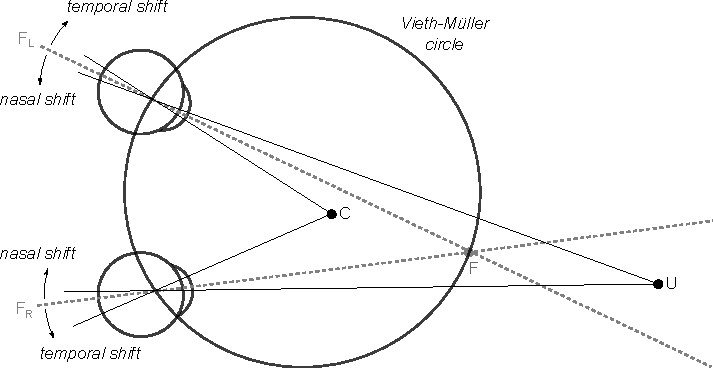
\includegraphics{disparity-classification}
  \caption[Disparity classification and the Vieth-M{\"u}ller circle.]{Disparity classification and the Vieth-M{\"u}ller circle. Adapted from \cite{howard2008seeing}.}
  \label{fig:dispclass}
\end{figure}

Based on figure \ref{fig:dispclass}, we can also introduce the concept of relative disparity between any two points. The relative disparity between $C$ and $U$ is simply defined as the difference between their absolute disparities, $\delta_{CU} = \delta_{C} - \delta_{U}$. Since $\delta  = \alpha - \beta$ (Fig. \ref{fig:geostereo}), the expression for relative disparity can be written as $\delta_{CU} = (\alpha_C-\alpha_U) - (\beta_C-\beta_U)$. Here, the absolute distance to the fixation point $F$ is no longer determinant in the measure of disparity.

\subsubsection{Disparity edges and occlusion}

As Leonardo da Vinci observed, opaque objects in the foreground occlude certain regions of the background depending on the visual axis of each eye. For instance, let us consider a central fronto-parallel opaque surface closer to the observer in relation to a particular surround (Fig. \ref{fig:monocc}a), in which the occluded regions of the background in each eye may be common or exclusive. The areas occluded in both retinal images are known as binocular occlusions, and are naturally not visible to the observer (Fig. \ref{fig:monocc}a, dark turquoise area). Conversely, regions that are exclusively occluded in one of the retinal images are known as monocular occlusions (Fig. \ref{fig:monocc}a, cyan and pink areas). Because monocular occluded regions, also known as \textit{unpaired} regions, are not present in both eyes, there is no possible binocular correspondence between them. Hence, the classical definition of binocular disparity cannot be applied to visual elements in these regions. However, the retinal position of monocular occluded areas in relation to the central target (Fig. \ref{fig:monocc}, blue) would be reversed if the surface was located further away from the observer in relation to the surround (Fig. \ref{fig:monocc}b). It thus follows that the presence of unpaired features is a stereoscopic cue to depth. Nakayama and Shimojo \cite{Nakayama:1990fc} intuitively explain the problem at hand: the pattern of unpaired regions in the retinal images is associated with a \textit{depth constraint zone}---due to the geometry of occlusions, a given unpaired feature is a projection of an object that can only be located in a particular region in space defined by visibility lines.

\begin{figure}
  \centering
  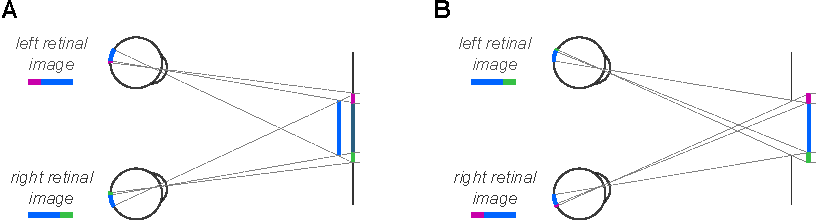
\includegraphics[width=14cm, keepaspectratio]{monocular-occlusion}
  \caption[Geometry of stereoscopic occlusions.]{Geometry of stereoscopic occlusions. Monocular regions (green and pink) are exclusively captured by the left and right eyes. The position of the monocular regions in relation to the target depends on eye-of-origin information, and is diagnostic of depth (compare A and B).}
  \label{fig:monocc}
\end{figure}

In this section, I have explained how differences between the left and right retinal images relate to distance between objects in 3-d space. In the next section, I will review behavioural observations which show that humans and other mammals make use of interocular image differences for depth perception.

\subsection{Stereoscopic depth perception}

We have previously seen how the horizontal separation of the eyes gives rise to binocular disparities. But can humans estimate depth based on such disparities? Charles Wheatstone provided the first evidence in support of this idea: he reported that if the two-dimensional perspective views of a solid object (as seen from the vantage point of each eye) were presented separately to the left and right eyes, observers experienced the three-dimensional configuration of that object \cite{Wheatstone:1838xf}. Whether binocular disparity alone could support depth perception was unknown, because Wheatstone's experiments lacked obviation of other cues to depth. Later, Heinrich Dove reported that stereopsis occurred for very brief stimulation periods before any eye movements could occur \cite{Dove1841,Dove1860}, suggesting that humans do not require vergence and accommodation cues to extract depth information from binocular disparity. Although initially in disagreement, Franciscus Donders later acknowledged that changes in vergence were not necessary in order to extract depth information from binocular disparity \cite{Donders1867}.

Apart from vergence and accommodation, Wheatstone's experiments also lacked obviation of other cues to depth. As Wheatstone defined it, the stimuli used in the experiment were the perspective views of a real object \cite{Wheatstone:1838xf}. Therefore, perspective alone could be use as a cue to depth. Evident in Wheatstone's report \cite{Wheatstone:1838xf} (cf. figure N in Wheatstone's manuscript) are also additional signals that could be used for depth estimation, such as shading, occlusion and relative size cues. Thus, one question remained to be answered: are binocular disparities sufficient for depth perception?

A definitive answer to this question was given by Bela Julesz with the invention of the random-dot stereogram (RDS) \cite{JULESZ:1964ff}. This type of stimulus consisted of computer generated random patterns of black and white picture elements (pixels). Julesz generated stereoscopic pairs by displacing a given region of the stimulus in one eye in relation to the other. When binocularly fused, the displaced region of the stimulus is perceived closer or further away in relation to the remaining region of the stereogram (Fig. \ref{fig:rds}). Thus, the random-dot stereogram provided means of rendering three-dimensional structures by manipulating binocular disparity in isolation, without other visual cues to depth (e.g. perspective, occlusion, shading).

\begin{figure}
  \centering
  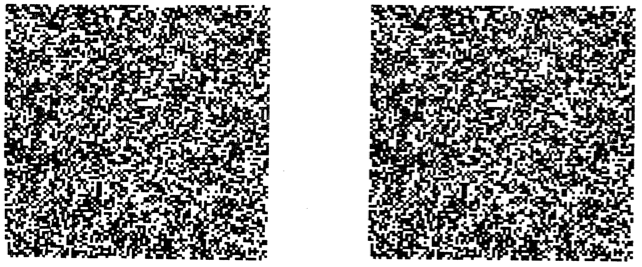
\includegraphics[width=10cm, height=6cm, keepaspectratio]{rds-julesz}
  \caption[Computer generated random-dot stereogram.]{Computer generated random-dot stereogram, invented by Bela Julesz. Adapted from \cite{JULESZ:1964ff}.}
  \label{fig:rds}
\end{figure}

\subsubsection{Stereopsis without correspondence} 

% Stereopsis is possible without exact feature correspondence
In his pioneering investigations, Julesz noted that depth percepts can emerge even in the absence of perfect correspondence between the left and right images \cite{JULESZ:1964ff}. In fact, even stereo pairs composed of very dissimilar features can effectively elicit a depth percept \cite{KAUFMAN:1964kx,KAUFMAN:1965vn,Mayhew:1976ys}, provided they have overlapping spectral content \cite{Mayhew:1976ys}. Stereopsis is also possible when a single feature is presented monocularly \cite{Kaye:1978os,Wilcox:2007zt}. Intuitively, these observations do not seem compatible with the detection of binocular disparities between corresponding features.

% Occluding contours
The study of stereopsis without correspondence is important because unpaired features occur frequently during natural stereoscopic viewing. For instance, an object in the foreground often causes occlusion of regions of the background in one eye, but not in the other (Fig. \ref{fig:monocc}). As a result, certain image features visible to one eye will often lack a correspondent in the fellow eye (i.e. they are unpaired).

% Humans do well with unpaired features
If stereopsis relies exclusively upon positional differences between corresponding regions, then unpaired binocular features should be irrelevant or even detrimental for depth perception. Surprisingly, humans appear to take advantage of the presence of unpaired features \cite{Gillam:1988lo, Shimojo:1988fk, Nakayama:1990fc, Shimojo:1990uq}. In certain circumstances, perception of depth in stereograms containing unpaired features emerges faster than in stereograms that lack them \cite{Gillam:1988lo}. Unpaired features that agree with occlusion geometry (Fig. \ref{fig:monocc}, see caption) escape rivalry and, as expected, are perceived as part of the background surface \cite{Shimojo:1990uq}. So long as they are ecological valid, unpaired features can be qualitatively and quantitatively used for depth perception, at least over a local range of up to 25-40 arcmin \cite{Nakayama:1990fc}, about half of the range of perceivable disparities \cite{TYLER:1975fu}. Due to Leonardo da Vinci's early observations on the relationship between occlusion and depth, stereopsis based on unpaired features became known as \textit{da Vinci stereopsis} \cite{Nakayama:1990fc}. 

% Unpaired vs Paired stereopsis - same or different mechanisms?
While it is accepted that unpaired information affects stereoscopic perception, a debate persists on whether conventional and \textit{da Vinci} stereopsis are supported by common mechanisms. Although it is unlikely that they rely exactly on the same processes \cite{Gillam:2003bh,Tsirlin:2012ys}, behavioural studies suggest that there is a considerable overlap. First, Pianta and colleagues observed cross-adaptation between the two types of stereopsis, and depth discrimination thresholds are strikingly similar \cite{Pianta:2003mz}. Second, depth from monocular occlusions can be biased by conventional disparity signals \cite{Tsirlin:2011bd}. Finally, depth perception elicited by brief monocular stimulation \cite{Kaye:1978os} can in theory be supported by a matching-to-fovea process \cite{Wilcox:2007zt}.

% Summary of this section
While stereopsis without correspondence is yet to be understood at the neural and perceptual levels \cite{Harris:2009qf}, it is clear that (i) lack of binocular correspondence occurs routinely under natural stereoscopic viewing \cite{Lawson:1967dq,Nakayama:1990fc,Anderson:1994fk,Anderson:1994qc}, and (ii) unpaired features can be perceived in depth \cite{Nakayama:1990fc, Shimojo:1990uq}. 

\subsubsection{Anticorrelated stereograms} \label{sssec: ards}

Perhaps the most enigmatic observations on stereopsis relate to anticorrelated stereograms --- stimuli in which elements are paired with inverted polarity across the half images (i.e. a bright element in one eye is paired with a dark element in the other eye, and vice-versa). Helmholtz had noticed that depth could be experienced in anticorrelated stereograms composed of thin lines, and the same holds for stereograms composed of bars \cite{Cumming:1998ib}. However, less clear observations have been made on anticorrelated random-dot stereograms \cite{Cogan:1993yr, Cumming:1998ib, Tanabe:2008gx, Doi:2011ku, Hibbard2014}. For very low dot densities, observers typically report a depth percept consistent with the binocular disparity imposed in the random-dot pattern \cite{Cogan:1993yr, Cumming:1998ib}, while for higher dot densities observers are usually unable to perceive depth \cite{JULESZ:1964ff, Hibbard2014}. To further complicate the matter, some observers seem to perceive reversed depth in anticorrelated stereograms \cite{Tanabe:2008gx, Doi:2011ku,Read:2000kx}, but only for very specific stimulus conditions (e.g. large disparity magnitudes \cite{Doi:2011ku}). As a result, the mechanisms that support depth perception based on anticorrelated stimuli remain elusive.


\section{Neural basis of stereopsis}  

% introduction - neural basis of perception
Understanding the relationship between neural activity and perception is a primary goal of sensory neuroscience. The last six decades have brought astounding progress to our understanding of how neurons in the brain encode information about the external world (i.e. neural encoding), and how these representations can be used to support perception (i.e. neural decoding). 

Characterizing what features drive individual neurons is an important step towards understanding neural encoding. With great success, neurophysiologists have been able to estimate spatial variations in brightness that best elicit neural responses in the retina \cite{Lettvin:1959gs,Levick:1967fk,Barlow:1972bh} and in primary visual cortex \cite{HUBEL:1959tz, HUBEL:1962ti, Hubel:1968hz}, generating insights into the mechanisms by which contrast and orientation are encoded in the brain. While neurons selective for binocular disparity have been found more than five decades ago \cite{Barlow:1967bs,Nikara:1968ys,Pettigrew:1968zr}, understanding encoding of binocular disparity has proven somewhat challenging.

In this chapter, I will briefly introduce the visual pathways and how they convey binocular information. I will then move on to describing disparity selectivity in early visual areas, and from there segue to higher cortical regions. I shall focus on non-human primates due to the evolutionary proximity to humans and the body of evidence available, briefly mentioning other species when relevant. However, I note that disparity selective neurons have been found across many other animal models, such as cat \cite{Barlow:1967bs}, owl \cite{Pettigrew:1976uq} and mouse \cite{Scholl:2013br}.

\subsection{Visual pathways and binocular information} \label{ssec:pathways}

Visual processing is hierarchically organized, whereby visual information travels through the brain via multiple tiers of massively parallel networks \cite{Felleman:1991kg} (Fig. \ref{fig:viscortex}). Visual information captured by the retina propagates via the lateral geniculate nucleus (LGN) primarily to primary visual cortex (V1), which in turn projects to a network of cortical areas organized according to a distributed hierarchy. Many of these areas are involved in stereopsis (Fig. \ref{fig:viscortex}B, pink labels), but their precise contribution to stereoscopic perception remains unknown.

\begin{figure}
  \centering
  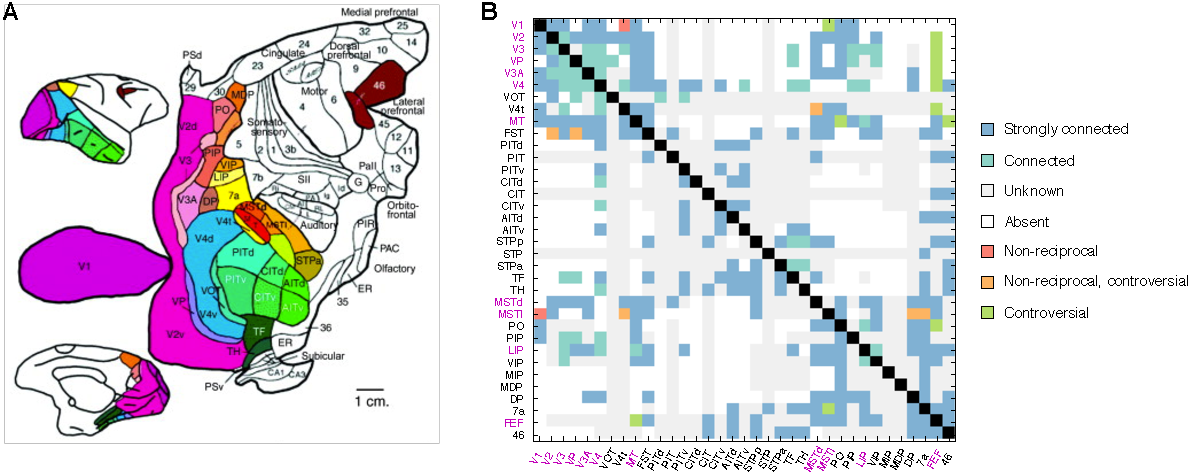
\includegraphics[width=14cm, keepaspectratio]{visual-cortex}
  \caption[Distributed cortical hierarchy.]{(A) map of cortical areas involved in vision in the macaque brain. (B) connectivity between the regions highlighted in color on panel A. Areas known to contain neurons selective for binocular disparity (summarized by Tsao and colleagues \cite{Tsao:2003lk}) are labeled in pink (in addition to these, certain regions in inferotemporal and parietal cortices also contain neurons selective for binocular disparity, as I will discuss below). Adapted from \cite{Felleman:1991kg}}
  \label{fig:viscortex}
\end{figure}

A prerequisite for encoding binocular disparity is to have access to the information captured by both eyes. Therefore, neurons that encode binocular disparity must be modulated by stimulation of either eye. In the retinae such neurons do not exist, and they are relatively rare in the LGN \cite{Howarth:2014aa,Dougherty:2018aa}, where the majority of the fibers remain segregated according to eye-of-origin. Up to this point, individual neurons are typically driven by stimulation of one eye, but not the other. Neural activity is then relayed from the LGN to V1 via axons terminating in layers 4C and 6 (a small proportion of cells, namely part of the koniocellular pathway, project to other layers) \cite{Nassi:2009hd}.

% Connectivity becomes increasingly complex after layer 4C
The signals propagated up to layer 4C are still largely segregated by eye-of-origin \cite{Hubel:1968hz}. Once in V1, the propagation of signals becomes more complex due to the abundance of feed-forward, horizontal and feedback connections \cite{Callaway1998, Nassi:2009hd, Harris:2013vn}. The major pathways can however be captured by a simple model both in the cat and the macaque---intermediate layers receive geniculate input and project mainly to superficial (supragranular) layers, which in turn project to extrastriate cortex. Neurons in superficial layers also project to deeper (infragranular) layers, which provide feedback projections to intermediate and superficial layers \cite{Callaway1998}. In the macaque, layer 4C receives the majority of geniculate input (and weaker projections to layer 6). Layer 4C projects mostly to superficial layers 2-4B, which in turn project to layer 5. Deep layers 5 and 6 provide strong feedback to layer 2-4B and 4C, respectively \cite{Callaway1998}.

% Binocularity in the different layers in V1
Neurons in layer 4 of V1 are still modulated by stimulation of one eye alone \cite{Hubel:1968hz} and are therefore not suitable for encoding binocular information. As we move towards supra- and infragranular layers the proportion of binocular neurons increases, with the highest proportion of binocular neurons being observed in supragranular layers 2/3 \cite{Hubel:1968hz, Poggio1972}. Therefore, neurons in supragranular layers of V1 seem to be the first with access to the necessary primitives to encode binocular disparity. At later stages of the cortical hierarchy, most neurons are binocular \cite{Burkhalter:1986fk, Maunsell:1987vn}.


\subsection{Disparity encoding in primary visual cortex}

% Introduction
Many neurons in primary visual cortex (V1) can be driven by stimulation of either the left or the right receptive fields \cite{HUBEL:1959tz,HUBEL:1962ti, Poggio1972}, and stimulating both eyes produces stronger responses than stimulating one eye alone \cite{HUBEL:1959tz,HUBEL:1962ti}. A possible mechanism for disparity encoding could then rely on slightly disparate receptive field positions in the left and right eye. Indeed, many binocular neurons in cat V1 are driven by binocular disparate regions \cite{Barlow:1967bs,Pettigrew:1968zr,Nikara:1968ys}, thus suggesting that they could support stereopsis. Disparity selective neurons were later found in macaque V1 \cite{Poggio:1977ys,Poggio:1981tg}, opening an avenue for more detailed investigations on how neurons in V1 may support stereopsis.

% Binocular simple and complex cells - summary
Based on the response to simple oriented stimuli, three major types of neurons were identified in V1: \textit{simple}, \textit{complex} and \textit{hypercomplex} cells \cite{HUBEL:1962ti,Hubel:1968hz}. Simple cells are either excited or suppressed by presenting dark or light oriented stimuli in particular regions of their receptive fields. Their receptive fields have clearly defined excitatory (ON) and inhibitory (OFF) subregions. Complex cells, on the other hand, do not seem to be modulated by the precise position of the stimuli within their receptive fields \cite{HUBEL:1962ti,Hubel:1968hz}. Both simple and complex cells have been implicated in stereopsis. To my knowledge, a relationship between hypercomplex cells and stereopsis has not been explicitly established. 

% binocular simple cells
Binocular simple cells are thought to perform initial encoding of binocular disparity \cite{Anzai1999,Cumming:1997fk,Ohzawa:1997bd,Ohzawa:1990cq,Ohzawa:1986xy}. Consistent with Barlow's hypothesis \cite{Barlow:1967bs}, early investigations suggested that simple cells encode disparity via differences in \textit{position} between the left and right receptive fields \cite{Heydt:1978mi,Ferster:1981kl} (Fig. \ref{fig:posphase}, left). However, subsequent studies revealed that the internal structure of the receptive field (i.e. the spatial arrangement of the ON and OFF subregions) varies considerably between the eyes \cite{DeAngelis:1991mb,Anzai:1997ud,Anzai:1999xd,Anzai:1999uq,Tsao:2003pi}. Such interocular differences can be well accounted for by differences in the phase parameter of a Gabor function --- hence the name \textit{phase shifts} \cite{DeAngelis1991,Prince:2002uq,Tsao:2003pi} (Fig. \ref{fig:posphase}, right). Thus, disparity encoding using both interocular position and phase, also know as hybrid encoding, provides the best description of disparity encoding in binocular simple cells V1 \cite{Anzai:1997ud,Anzai:1999xd,Prince:2002uq,Tsao:2003pi}.

\begin{figure}
  \centering
  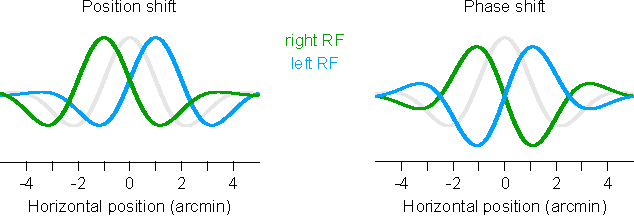
\includegraphics{position-phase}
  \caption[Receptive fields with interocular position and phase shifts.]{Left: receptive fields identical in structure but with different location in the two eyes can simply be related by a positional shift, and therefore they encode a positional disparity. Right: receptive fields with different internal structure in the two eyes can often be related by a shift in the phase parameter of a Gabor model. Blue and green lines represent the receptive field in the left and right eyes, respectively. Gray lines represent Gabors with zero position and zero phase shift.}
  \label{fig:posphase}
\end{figure}

% Binocular simple cells are selective to position within the RF
While binocular disparity modulates the firing rate of binocular simple cells, so does the overall stimulus position within the receptive field---even if disparity is kept constant \cite{Ohzawa:1990cq,Anzai:1997ud,Anzai:1999xd}. That is, two stimuli with equal disparities presented in slightly different positions within the receptive field may cause very different responses. Therefore, the activity of an individual binocular simple cell is not sufficient to signal the presence of particular binocular disparity.

% Properties of complex cells
As opposed to binocular simple cells, binocular complex cells are largely invariant to position within their receptive field, and are therefore better candidates for disparity detectors \cite{Ohzawa:1990cq}. The prevalent view was that complex cells inherit disparity selectivity by receiving excitatory input from multiple simple cells tuned to a particular preferred disparity \cite{Ohzawa:1986xy,Ohzawa:1990cq,Ohzawa:1997bd,Anzai1999}. It was also suggested that complex cells could integrate activity from other sources \cite{Livingstone:1999mp}---for instance, via direct geniculate inputs \cite{Archie:2000fk}---given the scarcity of binocular simple cells in the macaque brain \cite{Hubel:1968hz}.

There is now considerable evidence that individual complex cells receive inputs from neurons with a variety of disparity preferences. For instance, binocular complex cells can undergo adaptation by exposure to stimuli with non-preferred disparities \cite{Duong:2011fk}. They also seem to integrate activity over different positions, orientations and spatial frequencies \cite{Sasaki:2010pi,Baba:2015ij,Kato:2016fk}. Additionally, they receive suppressive input at opponent disparities \cite{Tanabe:2014ud,Tanabe:2011pt,Haefner:2008jg}. These generalized inputs are thought to improve selectivity of complex cells for binocular disparity \cite{Haefner:2008jg,Tanabe:2011pt,Kato:2016fk}.

% types of disparity selectivity
Can V1 complex cells then support stereoscopic perception? They are very diverse in their tuning properties, ranging from cells tuned to individual disparities, to cells tuned to a wide range of \textit{near} or \textit{far} disparities \cite{Poggio:1977ys,Poggio:1988ij,Prince:2002uq}. Thus, V1 complex cells provide a rich representation which could be used to support stereopsis. Although these cells are less selective than the perceptual system, a mechanism based on depth interpolation from a population of broadly tuned complex cells could in principle yield human-level stereoacuity thresholds \cite{Lehky:1990fk,Lehky1990}. Additionally, we know that complex cells are selective to disparity depicted in random-dot stereograms \cite{Poggio:1984mi,Poggio:1988ij}. Together, these findings suggest that V1 complex cells could play an important role in supporting stereoscopic perception. 

% Problems with complex cells 
However, there are significant deviations between the activity of complex cells and perceptual experience \cite{Cumming:1997ve, Cumming:2000vn}. For instance, anticorrelated RDS do not typically elicit perception of depth (see section \ref{sssec: ards}), but binocular complex cells still respond selectively to binocular disparities in these patterns \cite{Cumming:1997ve}. For many binocular complex cells, responses to disparity in anticorrelated stereograms are inverted and attenuated in relation to their responses to correlated stereograms \cite{Cumming:1997ve,Samonds:2013cs}. If binocular complex cells directly supported perception, an inversion in perceived depth would be expected, but this is hardly observed experimentally \cite{Cumming:1998ib,Hibbard2014}. Additionally, even when binocular images are correlated, binocular complex cells can signal disparities that do not match perception \cite{Cumming:2000vn,Nienborg:2006qo,Nienborg:2014fu}. Therefore, the activity of disparity complex cells in V1 seems insufficient to support stereoscopic depth perception, although it may provide a basis for fast corrective vergence eye movements \cite{Masson:1997jq}. Extrastriate cortex is thus expected to contribute to stereopsis.


\subsection{Disparity encoding in extrastriate cortex}

% areas involved
Disparity selective neurons are found throughout many extrastriate areas typically involved in vision \cite{Gonzalez:1998le,Neri:2005oq,Parker:2007nx}, such as V2 \cite{Hubel:1970dq,Poggio:1977ys}, V3/V3A \cite{Zeki:1978uf,Anzai:2011gb}, MT \cite{DeAngelis:1998df,DeAngelis:1999fk}, MST \cite{Eifuku:1999cr}, V4 \cite{Shiozaki:2012ys,Umeda:2007vn,Tanabe:2005qf,Watanabe:2002kx}, and inferior-temporal cortex \cite{Uka:2000cr,Janssen:2003fk,Janssen:2000oq,Janssen:1999nx}. In addition, neurons selective to binocular disparity are also found in anterior \cite{Verhoef:2015cz,Verhoef:2010gb,Srivastava:2009oa}, lateral \cite{Gnadt:1995tg,Genovesio:2004kl} and ventral \cite{Colby:1993oq} parietal areas, as well as in the frontal eye fields \cite{Ferraina:2000nx}, potentially for supporting visuomotor control.

% relation to perceptual experience
Contrary to V1, the activity of many neurons across different extrastriate areas is closely linked to stereoscopic perception. Choice related neural activity during depth judgments based on disparity has been found in V2 \cite{Clery:2015lh,Nienborg:2007ly,Nienborg:2006qo}, V4 \cite{Shiozaki:2012ys} and anterior intraparietal area\cite{Verhoef:2015cz}. Additionally, microstimulation and inactivation studies have established a causal link between neural activity and depth judgments in areas MT \cite{DeAngelis:1998df}, V2/V3 \cite{Smolyanskaya:2015ve}, V4 \cite{Shiozaki:2012ys} and inferior-temporal cortex \cite{Verhoef:2012dg}. Interestingly, responses to anticorrelated disparities are greatly attenuated in V4 \cite{Tanabe:2004mw} and absent at the level of inferior-temporal cortex \cite{Janssen:2003fk}---in stark contrast with neurons in V1 \cite{Cumming:1997ve}, MT \cite{Krug:2004fk} and MST \cite{Takemura:2001bd}.

Another point of differentiation between disparity encoding in primary and extrastriate visual cortex is the extent to which neurons are selectivity to relative disparities (i.e. differences between binocular disparities of different elements, such as the center and the surround of a circular RDS) \cite{Cumming:2000vn}. Neurons specialized for different forms of relative disparity can be found as early as in V2 \cite{Thomas:2002ud}, and to a higher degree in downstream areas V4 \cite{Umeda:2007vn}, MT \cite{Nguyenkim:2003if}, MST \cite{Roy:1992kc,Roy:1990hs}, and inferior-temporal cortex \cite{Janssen:1999nx,Janssen:2000oq}. These areas also seem to be specialized for different types of relative disparity. For instance, neurons in V2 and V4 respond well to relative disparities in center-surround configurations \cite{Thomas:2002ud,Umeda:2007vn}, while neurons in MT and CIP signal relative disparity in slanted surfaces \cite{Nguyenkim:2003if,Rosenberg:2013fk}. Specialization for relative disparity in areas V3 and V3A is controversial --- while neuroimaging studies suggest that V3/V3A are correlates of depth perception based on relative changes in disparity \cite{Backus:2001ly,Tsao:2003lk,Ban:2015cr}, neurophysiological data suggests no selectivity for relative disparity, at least for center-surround stimulus configurations \cite{Anzai:2011gb}.

The precise contribution of extrastriate visual areas for disparity processing remains unknown. They may be arranged into parallel hierarchical streams with different functional roles \cite{Tyler:1990gb}. For instance, lesions show that the parvocellular and magnocellular pathways subserve different roles in stereopsis: damage to the parvocellular pathway impairs fine stereopsis, with no impact on coarse depth judgments, while damage to the magnocellular pathway leaves fine stereopsis unaffected \cite{Schiller:1990sh}. It is therefore possible that different aspects of stereopsis are segregated according to these pathways \cite{Tyler:1990gb}.

A similar, potentially related, segregation in stereoscopic processing may also exist across ventral and dorsal streams \cite{Parker:2007nx}. For instance, dorsal area MT may underlie fast, coarse depth perception \cite{Uka:2003uq, Uka_2006}, and does not support fine disparity discrimination \cite{Uka_2006}. Parietal areas also show preference for fast, coarse depth perception \cite{Srivastava:2009oa}. Conversely, areas along the ventral stream show sharp selectivity for fine relative disparities that compose complex 3D shapes \cite{Watanabe:2002kx,Umeda:2007vn,Shiozaki:2012ys,Verhoef:2012dg,Janssen:2000oq,Janssen:2003fk}. This suggests that the ventral stream may extract fine disparities more suitable for perception of 3D shape, while the dorsal stream may process coarse disparities for visually guided action \cite{Parker:2007nx, Roe_Parker_Born_DeAngelis_2007}. Within the dorsal stream, different pathways are likely to coexist: for instance, sensory signals can propagate to parietal cortex indirectly via V3A \cite{Orban:2006kn}, while they are conveyed in parallel to MT via direct and indirect input from V1. This indirect pathway to MT, particularly via V2/V3, is thought to be important for depth judgments \cite{Ponce:2008km,Smolyanskaya:2015ve}.

\subsubsection{Cortical organization for binocular disparity}

% this needs work probably
In many species, V1 neurons are systematically organized along the cortex, whereby they cluster in columns with similar eye dominance and preferred orientation \cite{Hubel:1974sv,Wiesel:1974am,Hubel:1968hz,HUBEL:1962ti,Hubel:1978zt,Hubel:1969il}. While the precise role of cortical columns remains unclear \cite{Horton:2005hb}, it is possible that emergence of perceptual related activity requires columnar organization \cite{Nienborg:2014fu}. In V1, cortical clustering according to preferred disparity is only weak \cite{LeVay:1988ve,Prince:2002cr}, and is possibly driven by a correlation between preferred disparity and eye dominance \cite{Poggio:1977ys,LeVay:1988ve}.

By contrast, some extrastriate areas display cortical organization for binocular disparity. The first signs of clear organization for binocular disparity are found in V2: disparity selective neurons are clustered in the thick stripes of primate V2 \cite{Hubel:1987ly}, and seem organized according to disparity preference \cite{Hubel:1970dq, Chen:2008vn}. In the cat, cortical organization for binocular disparity has also been observed \cite{Kara:2009fk}. Further down the dorsal stream, columnar organization for binocular disparity is found in areas V3/V3A \cite{Adams:2001wt, Anzai:2011gb, Yeagle_Lafer-Sousa_Conway_2013} and MT \cite{DeAngelis:1999fk}.
 
\section{Theory and physiological computation} 

\subsection{Theory of stereoscopic perception}


% We still need a theory of stereopsis - what are we looking for? - what is involved (vergence, etc)? 
Stereopsis operates under very general conditions. We perceive depth in highly structured images \cite{Wheatstone:1838xf}, but also in random-dot patterns which lack the texture and form statistics that characterize natural images \cite{BLTJ:BLTJ3954}. Although stereopsis relies on positional differences between the left and right retinal images, binocular correspondence is not strictly necessary to elicit depth percepts \cite{KAUFMAN:1965vn,Mayhew:1976ys,Kaye:1978os,Nakayama:1990fc}. Moreover, we achieve stable depth percepts although fusion and vergence are in constant interaction \cite{Sperling:1970ys,Masson:1997jq}. Elaborating theories of stereopsis that encompass these different aspects is challenging but necessary to guide future experimentation.

% two approaches: perception- vs computation-driven
Early theories of stereopsis emerged within the field of experimental psychology \cite{hering1977theory,koffka1935principles,Boring:1942bs,ogle1950researches,woodworth1954experimental}. They had been developed around unexplained psychophysical observations, which could in a way tell us something about how the brain operates. Take, for instance, the problem of the primitives of stereopsis. What visual features does the brain use to estimate depth from binocular disparity? To answer this question, one could experimentally control the features available to the visual system, and then evaluate whether stereopsis is achieved \cite{KAUFMAN:1965vn,KAUFMAN:1964kx,Mayhew:1976ys}.

An alternative approach pioneered by David Marr focused on computational goals instead (here estimating depth from disparity). The \textit{Marrian} logic is to depart from the computation that needs to be done to solve a particular task, identify constraints, and propose an algorithm to solve the computational problem. This approach is agnostic as to how the solution is implemented in the brain, and focuses on the nature of the computation that the system must perform \cite{Chomsky:1965kx,Marr:1976dq}. The computation, rather than the precise circuitry implementing it, can then be the used to relate neural activity to perception \cite{Carandini:2012ce}. While some concerns exist with respect to this approach \cite{Anderson:2015fu}, it stimulated a wide variety of theorists to propose quantitative models of stereopsis.

% % -- solving the stereo-correspondence problem
Let us consider the problem of computing a binocular disparity. To do so, it is necessary to determine the correspondence between visual features present in the left and right retinal images---this is known as \textit{the stereo-correspondence problem}. This is a challenging computation because images may contain many self-similar elements: in random-dot stereograms, for instance, each pixel in one image can be matched with many similar pixels in the other image. 

% - matching primitives
In looking for a solution to the stereo-correspondence problem, perhaps the first consideration pertains to the substrate of matching, also known as matching primitives. What are the elements for which correspondence is to be established? Object recognition is not necessary for stereopsis, as demonstrated by Julesz' random-dot stereogram \cite{BLTJ:BLTJ3954}, so stereo matching does not operate on object elements or parts. Instead, matching should occur at the level of relatively simple features. One possibility is that the visual system matches very low-level features, such as the brightness of simple dot elements \cite{Marr:1976dq,MAYHEW1981349}. Alternatively, the visual system may operate on so-called zero crossings---areas where contrast polarity shifts from positive to negative and vice-versa \cite{Marr:1979lh,Grimson:1981bs}---or more complex features such as average brightness or contours \cite{KAUFMAN:1964kx,KAUFMAN:1965vn,Ramachandran:1973kl,Ramachandran:1976mi}. Increasing the complexity of the primitives has the advantage of reducing the difficulty of the stereo-correspondence problem, but may also mean that simple features are left unmatched \cite{Marr:1979lh,MAYHEW1981349,Anderson:1994fk}. 

% - global stereopsis
Another important issue is how the brain goes from a set of matching possibilities to a coherent solution, known as global stereopsis. Again, this problem is fairly evident in random-dot stereograms: a variety of equally good matches is available locally, and the correct match can only be determined by considering global information \cite{Julesz:1971uq}. To deal with this problem, many theories of stereopsis use disparity detectors that are densely interconnected across space and depth \cite{Julesz:1971uq,Marr:1976dq,Sperling:1970ys,Prazdny:1985vn,Nelson:1975oq}, thus ensuring global support. One potential problem with this approach is that it requires a very large number of connections. It is however possible to achieve global support with iterative local computations, which require a much smaller number of connections \cite{export:75622}. These theories suggest that the visual system may arrive at a global solution via local iterative computations and/or multi-scale interactions.

% - constraints
The stereo-correspondence problem can also be simplified by imposing constraints derived from ecological considerations. For instance, disparity in surfaces usually varies smoothly, so a constraint may be imposed that discards large local variations in disparity. In practice, this can be implemented by local excitation in the spatial domain \cite{Sperling:1970ys,Nelson:1975oq,DEV1975511,Marr:1976dq} (Fig. \ref{fig:correspondence}a, red elements). A constraint may also be imposed in the rate of change of disparity across space \cite{Pollard01081985} (Fig. \ref{fig:correspondence}b), or in local incoherence within different depth fields \cite{Prazdny:1985vn}. The stereo-correspondence problem can also be ameliorated by considering detectors tuned to different orientations and spatial frequencies \cite{Marr:1979lh}. Finally, inhibitory interactions between different disparity detectors can impose uniqueness on the disparity solution \cite{Sperling:1970ys,Nelson:1975oq,DEV1975511,Marr:1976dq}. The solution is usually arrived at using cooperative interactions between different detectors \cite{Marr:1976dq,Marr:1979lh}.


\begin{figure}
  \centering
  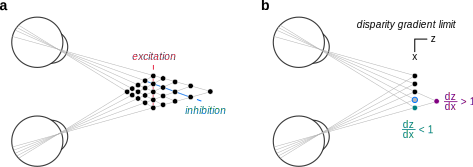
\includegraphics[width=14cm, keepaspectratio]{corr-problem}
  \caption[The stereo-correspondence problem.]{The stereo-correspondence problem and two strategies to overcome it. (A), continuity can be promoted by local excitation along the fronto-parallel direction. Inhibition along different lines of sight implement a uniqueness constraint. (B) elimination of a false match using the disparity gradient limit. In this example, one of two dots must be selected (turquoise or purple dot). The rate of change of disparity as a function of fronto-parallel displacement (with respect to the nearest match, blue dot) is used to discard false matches. Values greater than unity are considered violations of the disparity gradient limit, and such matches are therefore rejected. The criterion is based on perceptual observations \cite{Burt:1980ys}.}
  \label{fig:correspondence}
\end{figure}

% - beyond matching in stereo-correspondence
These views make a central assumption that disparity can be extracted after matching corresponding features on the basis of their similarity. However, as I have alluded to above, it has been shown that human stereopsis operates on displays for which no exact correspondence can be achieved \cite{Kaye:1978os,Mayhew:1976ys}, and that it can even be improved by introducing features that are only present in one half-image \cite{Gillam:1999il,Anderson:1994fk,Nakayama:1990fc,Shimojo:1990uq,Gillam:1988lo}. Thus, it has been suggested that more elaborate theories --- that do not rely exclusively on matching --- are needed to explain behavioural observations. One alternative theory is that the visual system explores dissimilarities between the half-images as a binocular cue to depth, possibly exploring three-dimensional ecological constraints \cite{Anderson:1994fk,Nakayama:1990fc,Shimojo:1990uq}. This view has perhaps not received enough attention, but it is nevertheless plausible. Half-occluded regions are a cue to the presence of occluding contours, and therefore identifying such regions is informative for inferring the depth structure of a scene \cite{belhumeur1992bayesian,belhumeur1996bayesian,Anderson:1994qc,Anderson:1994fk,anderson1995theoretical}. From a computational standpoint, an optimized system should be able to explore this dependency to estimate depth from binocular disparity. Recent theories propose that such occlusions are explicitly detected by a group of cells in the visual system \cite{Tsirlin2014}, a prediction that is yet to be tested.   

% - the role of the eyes
Finally, it is also important to consider the close relationship between stereopsis, vergence and accommodation. For instance, it is known that even very brief stereoscopic presentation elicits rapid, corrective vergence eye movements \cite{Masson:1997jq}, and that disparity and accommodation dependent jointly affect eye-movements that facilitate binocular fusion \cite{Maiello:2014nu}. Although vergence eye movements have been suggested to help in bringing large disparities into correspondence \cite{Marr:1979lh,Grimson:1981bs}, few have attempted to relate stereopsis to the oculomotor system as whole \cite{Sperling:1970ys}.

% - conclusion
The theoretical models above are either inspired or constrained by observations taken from early neurophysiological experiments. They consider general principles of cortical circuits, such as the existence of excitatory-inhibitory interactions \cite{Sperling:1970ys,DEV1975511,Marr:1976dq} and the arrangement into cortical columns \cite{Nelson:1975oq}. However, limited data on the properties of disparity selective neurons was available at that time. In the next section, I will review models of stereoscopic vision that aim to describe what the brain computes in order to estimate depth from binocular disparity.

\subsection{Physiological models}


The theoretical work hereto mentioned provides insights on the problems associated with stereoscopic perception. But what exactly does the visual system do to extract depth from binocular disparity? What are the neural computations involved? To answer this question, it is first important to characterize the computational abilities of neurons, i.e. the kind of computations that neurons are able to perform. 

Significant advances in this quest have been made in the visual system, particularly in the retina \cite{Enroth-Cugell:1966zr}, LGN \cite{Shapley:1975aa} and V1 \cite{Movshon:1978dq}. For instance, simple cells in V1 (as X/P cells in the retina and LGN) behave quite linearly for a wide range of contrast energy, and their response can be well predicted on the basis of spatial summation over the receptive field followed by a rectification step that ensures non-negative firing rates \cite{Movshon:1978dq} (Fig. \ref{fig:earlymodels}A). Thus, these cells can be modeled as \textit{linear-nonlinear} units, whereby the predicted activity of the cell is given by linear filtering of the stimulus by the cell's receptive field, followed by a static nonlinearity. To account for responses to high contrast stimuli, which deviate from the linear behaviour \cite{Maffei:1973aa}, subsequent divisive normalization is required \cite{Carandini97linearityand}.

\begin{figure}
  \centering
  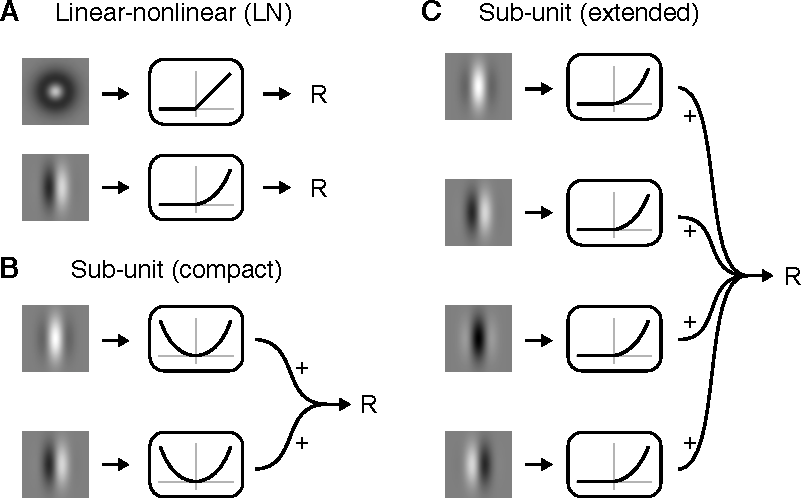
\includegraphics{early-models}
  \caption[Models of physiological computation in early visual areas.]{Simple models of physiological computation in early visual areas. (A) according to linear-nonlinear models, the response of a cell can be predicted by linear filtering by the receptive field (e.g., a centre-surround field as seen in the retina, or an oriented Gabor field as seen in V1) followed by a nonlinearity. (B, C) Subunit models combine the activity of simple cells (modeled as linear-nonlinear units) with receptive fields in quadrature-phase. The models represented in B and C are identical in their response, but they differ in their implementation. Panel B shows a compact representation where ON and OFF responses are computed by the same subunit, whereas panel C shows an extended representation where ON and OFF responses are computed by separate subunits.}
  \label{fig:earlymodels}
\end{figure}

Complex cells in V1 (as Y cells in the retina \cite{Enroth-Cugell:1966zr,Hochstein:1976ly} and LGN \cite{Shapley:1975aa}), on the other hand, deviate markedly from the linear-nonlinear model \cite{Movshon:1978bh}. For instance, complex cells exhibit sustained responses to sweeping oriented lines, which effectively means that their response is not strongly affected by the position of the line within the receptive field. One possible mechanism to achieve position invariance relies on pooling the responses of simple cells (so-called subunits) with different spatial arrangements of ON-OFF receptive field regions \cite{HUBEL:1962ti,Hochstein:1976ly,Movshon:1978bh}. The response of a complex cell can thus be modeled by pooling the responses of multiple linear-nonlinear units, each representing one simple cell (Fig. \ref{fig:earlymodels}B,C). Subunit models are typically instantiated such that the receptive fields of the subunits are arranged in quadrature-phase, which ensures position invariance with the receptive field and equal responses to increments and decrements of light.

Following these building blocks of neural computation, Ohzawa and colleagues proposed a model that shaped the following two decades of investigations on stereopsis --- the binocular energy model \cite{Ohzawa:1990cq}. Using a subunit model, Ohzawa and colleagues proposed that disparity selective complex cells combine the output of four binocular simple cells with receptive fields in quadrature-phase  (Fig. \ref{fig:dem}), with disparity selectivity emerging due to interocular differences between the left and right receptive fields. The original form of the binocular energy model includes a rectifying non-linearity at the output of the simple cells (Fig. \ref{fig:dem}), but modified versions of the model usually include additional nonlinearities (as I shall discuss later).

\begin{figure}
  \centering
  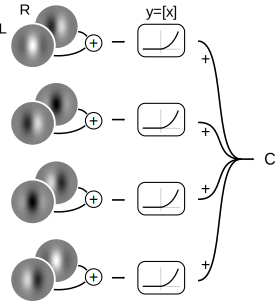
\includegraphics{dem-arch}
  \caption[The architecture of the binocular energy model.]{The architecture of the binocular energy model \cite{Ohzawa:1990cq}. For each subunit, the left and right images are convolved with the corresponding receptive fields. The filtering output for the left and right eyes are then summed (binocular summation) and the result is rectified. The rectified output of each subunit is then combined into an output complex cell. Modifications to the original energy model typically rely on additional nonlinearities at different stages of the model (e.g. before binocular summation).}
  \label{fig:dem}
\end{figure}

Let us define $B$ as the set of responses of four simple cells in quadrature-phase, $B=\{b_{0}, b_{\pi/2}, b_{\pi}, b_{3\pi/2}\}$, where the subscripts denote the phase of the Gabor receptive fields. Formally, the response of a complex cell, $c$, is given by:
\begin{equation}
c = \sum_{b \in B} b.
\label{eq:complex}
\end{equation}

In turn, the response of a simple cell is given by filtering the left and right images by the corresponding (i.e. left and right) receptive fields, summing the respective results, and applying a rectifying non-linearity. The response of a simple cell can thus be written as:

\begin{equation}
b = [l + r]_{+}^2,
\label{eq:simple}
\end{equation}

where $l$ and $r$ are given by the dot product between the left/right input images and the left/right receptive fields, respectively, and $[.]_+$ denotes rectification. As mentioned earlier, the units of the energy model are arranged into two ON-OFF pairs. Thus, one can compute the aggregated response of two subunits in a pair by replacing the half-rectified squaring non-linearity by full-rectification. Thus, the response of a complex cell can be equivalently expressed by

\begin{eqnarray}
c = (l_{0} + r_{0})^2 + (l_{\pi/2} + r_{\pi/2})^2,
\end{eqnarray}

where the subscripts again denote the phase of the Gabor receptive fields. By expanding the quadratic terms, it becomes clear that the response of a given complex cell depends not only on binocular interactions between the left and right images, but also on monocular information alone:  

\begin{eqnarray}
c = l_{0}^2 + r_{0}^2 + 2l_{0}r_{0} + l_{\pi/2}^2 + r_{\pi/2}^2 + 2l_{\pi/2}r_{\pi/2}.
\label{eq:complexEx}
\end{eqnarray}

Equation \ref{eq:complexEx} is useful to understand how the binocular energy model works and what are its limitations. The response of the complex cell depends on six terms, only two of which are modulated by binocular information (the cross terms). Varying the disparity of the stimulus affects the binocular terms, but the quadratic terms are unaffected because they do not depend on binocular information.

Two important conclusions can be taken from this equation. First, the response of the complex cell depends on monocular contrast --- for a given stereo image pair, increasing the contrast will cause an increase of the monocular responses $l$ and $r$. Second, selectivity for disparity is supported by the cross-terms $2lr$. Thus, the complex cell's response is modulated by the covariance between the left and right inputs. As a result, by replacing one of the images by its negative, equation \ref{eq:complexEx} explains why the binocular energy model produces inverted responses to anticorrelated stimuli --- the monocular terms remain unaffected, but the sign of the cross-term is inverted.

Equation \ref{eq:complexEx} demonstrates that the binocular energy model is too linear to account for the attenuation in response to anticorrelation \cite{Cumming:1997ve}. A significant amount of work in the last two decades has focused on modifying the energy model in order to account for this effect. A very simple way to explain the attenuation is the introduction of a threshold or non-linearity to the output of the complex cell \cite{Lippert:2001fk, Read:2002kx}. However, this solution explains attenuation exclusively for tuned-excitatory cells and does not generalize to \textit{near}, \textit{far}, or \textit{tuned-inhibitory} cells \cite{Read:2002kx}. Another alternative is to introduce additional non-linearities before binocular combination, and modify the binocular summation stage of the model \cite{Read:2002kx,Read:2003ij}. Finally, combining opponent excitatory-suppressive inputs from multiple subunits \cite{Haefner:2008jg, Tanabe:2008lo} can also lead to attenuated responses to anticorrelated stimuli.

%% resolving ambiguities (false matches)
Besides the difficulties in explaining properties of neurons, the classical binocular energy model also performs sub-optimally when it comes to computation. In the binocular energy model, the computation of depth from disparity is usually based on a maximum energy criterium, whereby the preferred disparity of the complex cell that responds the most is taken to be the predicted disparity of the stimulus \cite{Qian:1997bu,Qian:1994:CSD:1362347.1362350,Read:2002kx}. However, it has been shown that the binocular energy model does not recover the correct disparity consistently: it very often --- approximately 70\% of the time \cite{Read:2007nx} --- produces spurious energy peaks at incorrect disparities, usually referred to as false matches \cite{Fleet:1996tq,Read:2007nx}.

One possible mechanism to abolish false matches is to pool the output of the energy model across multiple orientations and spatial scales \cite{Fleet:1996tq}. This is effective because false peaks in energy occur at different disparities across different orientations and spatial scales, so they are attenuated by pooling. A more complex algorithm to eliminate false matches relies on the energy responses of detectors with a wide range of position and phase shifts, which can disambiguate the correct disparity in the stimulus \cite{Read:2007nx}.

% alternatives to the binocular energy model
Although physiological models of stereopsis have been gravitating around the binocular energy model, it remains unclear whether or not disparity selective complex cells receive input from simple cells, as suggested by subunit models. In fact, based on neural recordings from macaque primary visual cortex, Livingstone and Tsao found no evidence in support of this idea \cite{Livingstone:1999mp}. An alternative possibility is that disparity selective complex cells receive direct inputs from alternating layers of the LGN, with non-linear binocular integration happening at the dendritic level \cite{Archie:2000fk}. Although this model departs from the mechanistic account provided by the energy model, the computations implemented are closely related---this model too relies on a linear-nonlinear binocular summation followed by integration of the activities of four subunits (in this case LGN efferents). The repertoire of neurophsysiological observations available to date is not yet sufficiently large to definitively tease apart the mechanisms by which disparity selectivity arises in V1 complex cells.


\section{Thesis Overview} 

In the following chapters, I shall address three aspects of neural stereoscopic processing that remain poorly understood. I will start by looking at the computational mechanisms that may underly early disparity processing in the brain. The goal is to identify and describe a mechanism optimized to extract depth from binocular disparity, ideally based on natural images, and that can reproduce relevant neurophysiological and psychophysical data.

I will then examine to which extent neural selectivity for disparity in primary visual cortex limits stereoscopic perception. In particular, inspired by predictions of the modelling work presented in Chapter 2, Chapter 3 explores the psychophysical consequences of encoding binocular disparity optimally. The aim is to test if the properties of disparity selective neurons in V1, as reported in Chapter 2, constrain stereoscopic depth perception.

Next, I will turn to the characterization of higher brain regions that are thought to be specialized for binocular disparity in humans. Previous neuroimaging work suggests that areas in dorsomedial visual cortex are closely related to depth perception \cite{Backus:2001ly,Tsao:2003lk,Preston:2008dg}. I will examine these areas in greater spatial detail (for neuroimaging standards) using ultra-high field (7 Tesla) functional magnetic resonance imaging, with the main objective of testing for evidence of specialized cortical organization.

I will end with an effort to examine the role of different cortical layers in stereopsis using layer-dependent functional magnetic resonance imaging with sub-millimeter resolution. The main goal is to establish the feasibility of this technique for testing stereoscopic processing in the human brain, laying out the foundation for future work on exploring the role of cortical layers in mediating interactions between the many visual areas involved in stereopsis.

%%% ----------------------------------------------------------------------


%%% Local Variables: 
%%% mode: latex
%%% TeX-master: "../thesis"
%%% End: 
